% Begin the document and set up the style of the document
\documentclass[a4paper]{article}

% Install the required packages for the document 
\usepackage{envmath}
\usepackage{esvect}
\usepackage{graphicx}
\usepackage{gensymb}
\usepackage{tikz}
\usepackage[mathcal]{euscript}
\usepackage{geometry}
\usepackage{enumitem}
\usepackage{mathtools}
\usepackage{graphicx}
\usepackage{amsmath}
\usepackage{amscd}
\usepackage{amssymb}
\usepackage{amsfonts}
\usepackage{harpoon}
\usepackage{pgf}
\usepackage{tikz}
\usepackage{mathrsfs}
\usepackage{asyalign}
\usepackage{physics}
\usepackage{enumitem}
\usepackage{xhfill}
\usepackage{accents}
\usepackage{cite}
\usepackage{url}
\usepackage[tableposition=top]{caption}
\usepackage{ifthen}
\usepackage[utf8]{inputenc}
\usepackage{tikz-3dplot}
\usetikzlibrary{patterns}
\usetikzlibrary{arrows}

% Page and style settings
\parskip=8pt
\parindent=0pt
% Right margin
\textwidth=6.25in
% Left margin
\oddsidemargin=0pt
\evensidemargin=0pt
% Bottom margin
\textheight=10in
% Top margin
\topmargin=-0.75in
\baselineskip=11pt
% end of page and other style settings

\renewcommand{\familydefault}{\sfdefault}


% Begin the text of the document
\begin{document}

% Begin the Title Page
\begin{titlepage}

\newcommand{\HRule}{\rule{\linewidth}{0.5mm}} % Defines a new command for the horizontal lines, change thickness here

\center % Center everything on the page
 
\textsc{\LARGE University of Sydney}\\[1.5cm] % Name of your university/college
\textsc{\Large MATH 1906}\\[0.5cm] % Major heading such as course name
\textsc{\large SSP}\\[0.5cm] % Minor heading such as course title

\HRule \\[0.4cm]
{ \huge \bfseries Assignment 3 - Chaos}\\[0.4cm] % Title of your document
\HRule \\[1.5cm]

\begin{minipage}{0.4\textwidth}
\begin{flushleft} \large
\emph{Author:}
Keegan Gyoery % Your name
\\
\emph{SID:}
470413467
\end{flushleft}
\end{minipage}
~
\begin{minipage}{0.4\textwidth}
\begin{flushright} \large
\emph{Lecturer:} 
Eduardo Altmann % Tutor's Name
\\
\emph{Seminar:}
New Law Annexe SR 442
Monday 4pm
\end{flushright}
\end{minipage}\\[4cm]

{\large \today}\\[3cm] % Date, change the \today to a set date if you want to be precise

\vfill % Fill the rest of the page with whitespace

\end{titlepage}

\pagenumbering{arabic}
%%%%%%%%%%%%%%%%%%%%%%%%%%%
%%%%%%%%%%%%%%%%%%%%%%%%%%%
%%%%%%%%%%%%%%%%%%%%%%%%%%%
%%%%%%%%%%%%%%%%%%%%%%%%%%%

Consider the dynamical system 
$$\displaystyle{x_{t+1} = f(x_t) = a - {x_t}^2 \dots \dots \dots \dots \dots (1)}$$
where $\displaystyle{t \in \mathbb{Z}}$ is the discrete time, $\displaystyle{a \in [0,2]}$ is a control parameter, and $\displaystyle{x_t \in [-2,2]}$ is the variable of interest.

\begin{enumerate}[label=\textbf{\arabic*.}]

	\item By definition, a fixed point belongs to a periodic orbit of period $n$ if $\displaystyle{x = f^{(n)}(x)}$, where $\displaystyle{f^{(n)}(x)}$ is the composition of the f with itself $n$ times. A periodic orbit of period $n$ is  composed by $n$ such points, $\displaystyle{x,f(x),f^{(2)}(x),\dots,f^{(n-1)}(x)}$.

	\begin{enumerate}
		\item In order to compute the fixed points that belong to the orbits of period 1 of the dynamical system $(1)$, we must use the above definition to begin the approach to finding these points. As a direct consequence of the definition, we set $\displaystyle{x_t = f^{(1)}(x_t)}$, in other terminology, $\displaystyle{x_t = f(x_t)}$. This definition leads to the following results for the fixed points of period 1 orbits of the aforementioned dynamical system.

		\begin{align*}
		x_t & = f(x_t)\\
		\therefore x_t & = a - {x_t}^2\\
		\therefore {x_t}^2 + x_t - a & = 0\\
		\therefore x_t & = \frac{-1 \pm \sqrt{1+4a}}{2}\\
		\end{align*}

		Thus the fixed points for the period 1 orbit of the dynamical system $(1)$, are:

		\begin{align*}
		x_t & = \frac{-1 + \sqrt{1+4a}}{2}\\
		x_t & = \frac{-1 - \sqrt{1+4a}}{2}\\
		\end{align*}


		\item Similarly, to compute the fixed points that belong to the orbits of period 2 of the dynamical system $(1)$, we again use the above definition to approach the problem of solving for the fixed points. As a result we get the result $\displaystyle{x_t = f^{(2)}(x_t)}$, which can be represented in the form, $\displaystyle{x_t = f(f(x_t))}$. Using the above result, we get the following fixed points for the period 2 orbits.

		\begin{align*}
		x_t & = f^{(2)}(x_t)\\
		\therefore x_t & = f(f(x_t))\\
		& = f(a - {x_t}^2)\\
		& = a - \left(a - {x_t}^2\right)^2\\
		& = a - \left(a^2 - 2a{x_t}^2 + {x_t}^4 \right)\\
		& = a - a^2 + 2a{x_t}^2 - {x_t}^4\\
		\therefore x_t & = a - a^2 + 2a{x_t}^2 - {x_t}^4\\
		\therefore {x_t}^4 - 2a{x_t}^2 + x_t + a^2 - a & = 0\\
		\end{align*}

		Due to the definition of fixed points, each subsequent orbit's stationary points are comprised of all the previous orbit's stationary points, and the points that are determined by the current orbit's periodicity. Thus, the above quartic has the fixed points from the period 1 orbit contained in it. Thus we know that the aforementioned quartic has the factor $\displaystyle{{x_t}^2 + x_t - a}$. Thus, using inspection, we are able to determine the factorisation of the quartic derived above.

		\begin{align*}
		{x_t}^4 - 2a{x_t}^2 + x_t + a^2 - a & = 0\\
		\therefore \left({x_t}^2 + x_t - a \right)\left({x_t}^2 - x_t - a + 1 \right) & = 0\\
		\end{align*}

		As mentioned above, the first factor gives the fixed points from the orbit with period 1, and thus we need not to examine that factor for solutions as we have already derived those. Thus the new fixed points that belong to the orbit of period 2 are as follows.

		\begin{align*}
		{x_t}^2 - x_t - a + 1 & = 0\\
		\therefore x_t & = \frac{1 \pm \sqrt{1 + 4(a - 1)}}{2}\\
		\therefore x_t & = \frac{1 \pm \sqrt{4a - 3}}{2}\\
		\end{align*}

		And thus the fixed points that belong to the orbits of period 2 of the dynamical system $(1)$, are:

		\begin{align*}
		x_t & = \frac{-1 + \sqrt{1+4a}}{2}\\
		x_t & = \frac{-1 - \sqrt{1+4a}}{2}\\
		\vspace{5mm}\\
		x_t & = \frac{1 + \sqrt{4a - 3}}{2}\\
		x_t & = \frac{1 - \sqrt{4a - 3}}{2}\\
		\end{align*}


		\item We are now required to compute the linear stability of all periodic orbits with periods 1 and 2, and as a consequence will be able to determine the subsequent intervals for which the orbits are stable and also unstable. We shall denote the values for which the orbits of period 1 and 2 lose stability by $a_1$ and $a_2$ respectively.

		\bigbreak

		Firstly, we will examine the stability of the periodic orbit with period 1. To do so, we will use the following process to derive the stable interval and $a_1$. We will use the notation $x^*$ to denote a point that satisfies the fixed point equation derived for a period 1 orbit above.

		\begin{align*}
		f(x_t) & = a - {x_t}^2\\
		\therefore x_{t+1} & = f(x^* + \delta x) \hspace{5mm} \text{where } \delta x \ll 1\\
		& \approx f(x^*) + \frac{df(x^*)}{dx^*} \cdot \left(x^* + \delta x - x^* \right)\\
		& = f(x^*) + \left(-2x^* \right) \cdot \left(x^* + \delta x - x^* \right)\\
		& = f(x^*) -2x^* \delta x\\
		& = x^* - 2x^* \delta x \hspace{5mm} \text{as } x^* \text{ is a fixed point and thus satisfies } x^* = f(x^*) \\
		\therefore \delta x^1 & = - 2x^*\delta x \hspace{5mm} \text{introducing the } \delta x^1 \text{ notation}\\
		x_{t+2} & = f(x^* + \delta x^1)\\
		& \approx f(x^*) + \frac{df(x^*)}{dx^*} \cdot \left(x^* + \delta x^1 - x^* \right)\\
		& = f(x^*) + \left(-2x^* \right) \cdot \left(x^* + \delta x^1 - x^* \right)\\
		& = f(x^*) -2x^* \delta x^1\\
		& = f(x^*) + \left(-2x^*\right) \left(-2x^*\delta x\right)\\
		& = f(x^*) + \left(-2x^* \right)^2 \\
		& = x^* + 4{x^*}^2 \hspace{5mm} \text{as } x^* \text{ is a fixed point and thus satisfies } x^* = f(x^*) \\
		\therefore x_{t+m} & = x^* + (-1)^m \left(2x^* \right)^m \delta x\\
		\end{align*}

		As a consequence of the definition $\displaystyle{x_{t+1} = f(x^*) + \frac{df(x^*)}{dx^*} \cdot \left(x^* + \delta x - x^* \right)}$, the following result occurs, $\displaystyle{x_{t+1} - x^* = \frac{df(x^*)}{dx^*} \cdot \left(\delta x \right)}$. Thus the derivative is characterised as follows.

		\begin{align*}
		x_{t+m} & = x^* + (-1)^m \left(2x^* \right)^m \delta x\\
		\therefore x_{t+m} - x^* & = (-1)^m \left(2x^* \right)^m \delta x\\
		\therefore \frac{df(x^*)}{dx^*} \cdot \left(\delta x \right) & = (-1)^m \left(2x^* \right)^m \delta x\\
		\therefore \frac{df(x^*)}{dx^*} & = (-1)^m \left(2x^* \right)^m\\
		\end{align*}

		In order to determine the interval upon which the periodic orbit of period 1 is stable, we must examine the following condition that governs stability, $\displaystyle{\left|f^{\prime}(x^*) \right| < 1}$.

		\begin{align*}
		\left|f^{\prime}(x^*) \right| & < 1\\
		\therefore \left|(-1)^m \left(2x^* \right)^m \right| & < 1\\
		\therefore \left|\left(2x^* \right)^m \right| & < 1\\
		\therefore \left|2x^* \right|^m & < 1\\
		\therefore \left|2x^* \right| & < 1\\
		\therefore \left|2\left[\frac{-1 \pm \sqrt{1+4a}}{2} \right] \right| & < 1\\
		\therefore \left|-1 \pm \sqrt{1+4a} \right| & < 1\\
		\therefore \left|-1 + \sqrt{1+4a} \right| & < 1\\
		\therefore -1 < -1 + \sqrt{1+4a} & < 1\\
		\therefore 0 < \sqrt{1+4a} & < 2\\
		\therefore 0 < 1 + 4a & < 4\\
		\therefore -1 < 4a & < 3\\
		\therefore \frac{-1}{4} < a & < \frac{3}{4}\\
		\therefore 0 \leq a & < \frac{3}{4} \hspace{5mm} \text{as } a \in [0,2]\\
		\end{align*}

		Thus the above interval is the interval upon which $a$ must lie for the orbit of period 1 to have stability. We were able to select the positive solution out of the two options as each solution, positive or negative would have returned the same interval within which stability resides. Thus an orbit of period 1 is stable $\displaystyle{\forall a \in \left[0,\frac{3}{4}\right]}$.

		\pagebreak

		In order to determine the intervals upon which instability occurs, the condition that governs instabilty, $\displaystyle{\left|f^{\prime}(x^*) \right| > 1}$ must be checked.
		
		\begin{align*}
		\left|f^{\prime}(x^*) \right| & > 1\\
		\therefore \left|(-1)^m \left(2x^* \right)^m \right| & > 1\\
		\therefore \left|\left(2x^* \right)^m \right| & > 1\\
		\therefore \left|2x^* \right|^m & > 1\\
		\therefore \left|2x^* \right| & > 1\\
		\therefore \left|2\left[\frac{-1 \pm \sqrt{1+4a}}{2} \right] \right| & > 1\\
		\therefore \left|-1 \pm \sqrt{1+4a} \right| & > 1\\
		\therefore \left|-1 + \sqrt{1+4a} \right| & > 1\\
		\end{align*}

		Once again we can select the positive solution as both solutions for the fixed point give the same results for the interval. Now in order to compute the values of $a$ where the dynamical system with a period 1 orbit is unstable, we must consider the two cases for the ineqaulity.

		\begin{align*}
		\therefore -1 + \sqrt{1+4a} & > 1\\
		\therefore \sqrt{1+4a} & > 2\\
		\therefore 1 + 4a & > 4\\
		\therefore 4a & > 3\\
		\therefore a & > \frac{3}{4}\\
		\end{align*}

		For the second case, we get the following result.

		\begin{align*}
		\therefore -1 + \sqrt{1+4a} & < -1\\
		\therefore \sqrt{1+4a} & < 0\\
		\therefore 1 + 4a & < 0\\
		\therefore 4a & < -1\\
		\therefore a & < \frac{-1}{4}\\
		\end{align*}

		As this unbounded interval lies completely outside the interval for $\displaystyle{a \in [0,2]}$, the second case is not counted in determining the interval for which the period 1 orbits are unstable. Thus the interval over which the period 1 orbits are unstable is $\displaystyle{a \in \left(\frac{3}{4},\infty \right)}$. Thus the value $a_1$, the parameter that dictates when period 1 orbits lose stability is $a_1 = \frac{3}{4}$.

		\pagebreak

		Now we will examine the stability of all periodic orbits with period 2, and thus derive the results for the intervals upon which the dynamical system is stable and unstable, and $a_2$. We will use the notation $x^{\dagger}$ to denote a point that satisfies a fixed point for a period 2 orbit of the dynamical system.

		\begin{align*}
		x_{t+2} & = f\circ f(x^{\dagger})\\
		& = f^{(2)}(x^{\dagger})\\
		\frac{d}{dx^{\dagger}}f^{(2)}(x^{\dagger}) & = \frac{df(f(x^{\dagger}))}{df(x^{\dagger})}\cdot \frac{df(x^{\dagger})}{dx^{\dagger}}\\
		& = f^\prime \left[x^{(2,+)} \right] \cdot f^\prime \left[x^{(2,-)} \right]\\
		& = \left[-2x^{(2,+)} \right] \left[-2x^{(2,-)} \right]\\
		\end{align*}

		The notation $\displaystyle{x^{(2,+)}}$ denotes the solution with the positive square root of the fixed point for an orbit with periodicity 2. Thus the results follow from the above notation definition.

		\begin{align*}
		x^{(2,+)} & = \frac{1 + \sqrt{4a - 3}}{2}\\
		x^{(2,-)} & = \frac{1 - \sqrt{4a - 3}}{2}\\
		\end{align*}

		Thus, continuing the derivation of the stability intervals and setting $\lambda$ equal to the continued derivation, the results below follow as a consequence.

		\begin{align*}
		\therefore \lambda & = \left[-2x^{(2,+)} \right] \left[-2x^{(2,-)} \right]\\
		& = \left[2\left[\frac{1 + \sqrt{4a-3}}{2} \right] \right] \left[2\left[\frac{1 - \sqrt{4a-3}}{2} \right] \right]\\
		& = \left[1 + \sqrt{4a-3}\right] \left[1 - \sqrt{4a-3}\right]\\
		& = 1 - (4a - 3)\\
		\therefore \lambda & = 4(1-a)\\
		\end{align*}

		Now examining the condition that governs the stability of the dynamical system with orbit of period 2, $\displaystyle{|\lambda| = \left|\prod_{i=1}^{m}f^\prime (x^{(m,\pm)})\right| < 1}$, we get the following results for the interval of $a$ that dictates stability for a period 2 orbit.

		\begin{align*}
		\therefore \lambda & = 4(1-a)\\
		\left|\lambda \right| & < 1\\
		\therefore \left|4(1-a) \right| & < 1\\
		\therefore -1 < 4(1-a) & < 1\\
		\therefore -1 < 4 - 4a & < 1\\
		\therefore -5 < -4a & < -3\\
		\therefore \frac{3}{4} < a & < \frac{5}{4}\\
		\end{align*}

		Thus the interval $\displaystyle{a \in \left(\frac{3}{4}, \frac{5}{4} \right)}$ is the interval in which $a$ must lie in order for the orbits of period 2 of the dynamical system to have stability. 

		\bigbreak

		Now in order to examine the intervals on which the orbits of period 2 are unstable, we must examine the governing restriction, $\displaystyle{|\lambda| = \left|\prod_{i=1}^{m}f^\prime (x^{(m,\pm)})\right| > 1}$. In doing so, we gain the following results.

		\begin{align*}
		\therefore \lambda & = 4(1-a)\\
		\left|\lambda \right| & > 1\\
		\therefore \left|4(1-a) \right| & > 1\\
		\end{align*}

		Now considering the first of two cases that arise from the inequality, we get the following result.

		\begin{align*}
		\left|4(1-a) \right| & > 1\\
		\therefore 4(1-a) & > 1\\
		\therefore 4 - 4a & > 1\\
		\therefore -4a & > -3\\
		\therefore a & < \frac{3}{4}\\
		\end{align*}

		Now considering the second of the two cases, we get the following result.

		\begin{align*}
		\left|4(1-a) \right| & > 1\\
		\therefore 4(1-a) & < -1\\
		\therefore  4 - 4a & < -1\\
		\therefore -4a & < -5\\
		\therefore a & > \frac{5}{4}\\
		\end{align*}

		As a result, we get the following two intervals upon which $a$ must lie for a periodic orbit of period 2 to be unstable. $\displaystyle{a \in \left[0,\frac{3}{4}\right)}$ and $\displaystyle{a \in \left(\frac{5}{4},2 \right]}$. The restrictions are as a consequence of the definition of $a \in [0,2]$. The value $a_2$, the parameter that determines when the orbit of period 2 loses is stability is $a_2 = \frac{5}{4}$.

		\pagebreak

		\item Firstly, the value of $a$ for the following graph must reside in the interval $a_1 < a < a_2$, governed by the bifurcation parameters $a_1 = \frac{3}{4}$ and $a_2 = \frac{5}{4}$. Thus we shall select $a = 1$ for the following plot. Now selecting two values, $x_0 = 0.25$, and $x_0^\prime = 0.5$ we get the following result for the $x_t$ vs $x_{t+1}$ graph. As it can be seen below, the value of $x_{t+1}$ oscillates between the values $0$ and $1$, as confirmed by iterations on a calculator. The black curve is the function $x_{t+1} = 1 -x^2$, and the blue line is given by the equation $x_{t+1} = x_t$. Thus its intersection point, $P$, with the curve gives the value for the stable point for orbits of period 1.

		\begin{center}
		\begin{figure}[h!]
		\caption{$x_t$ vs $x_{t+1}$}
			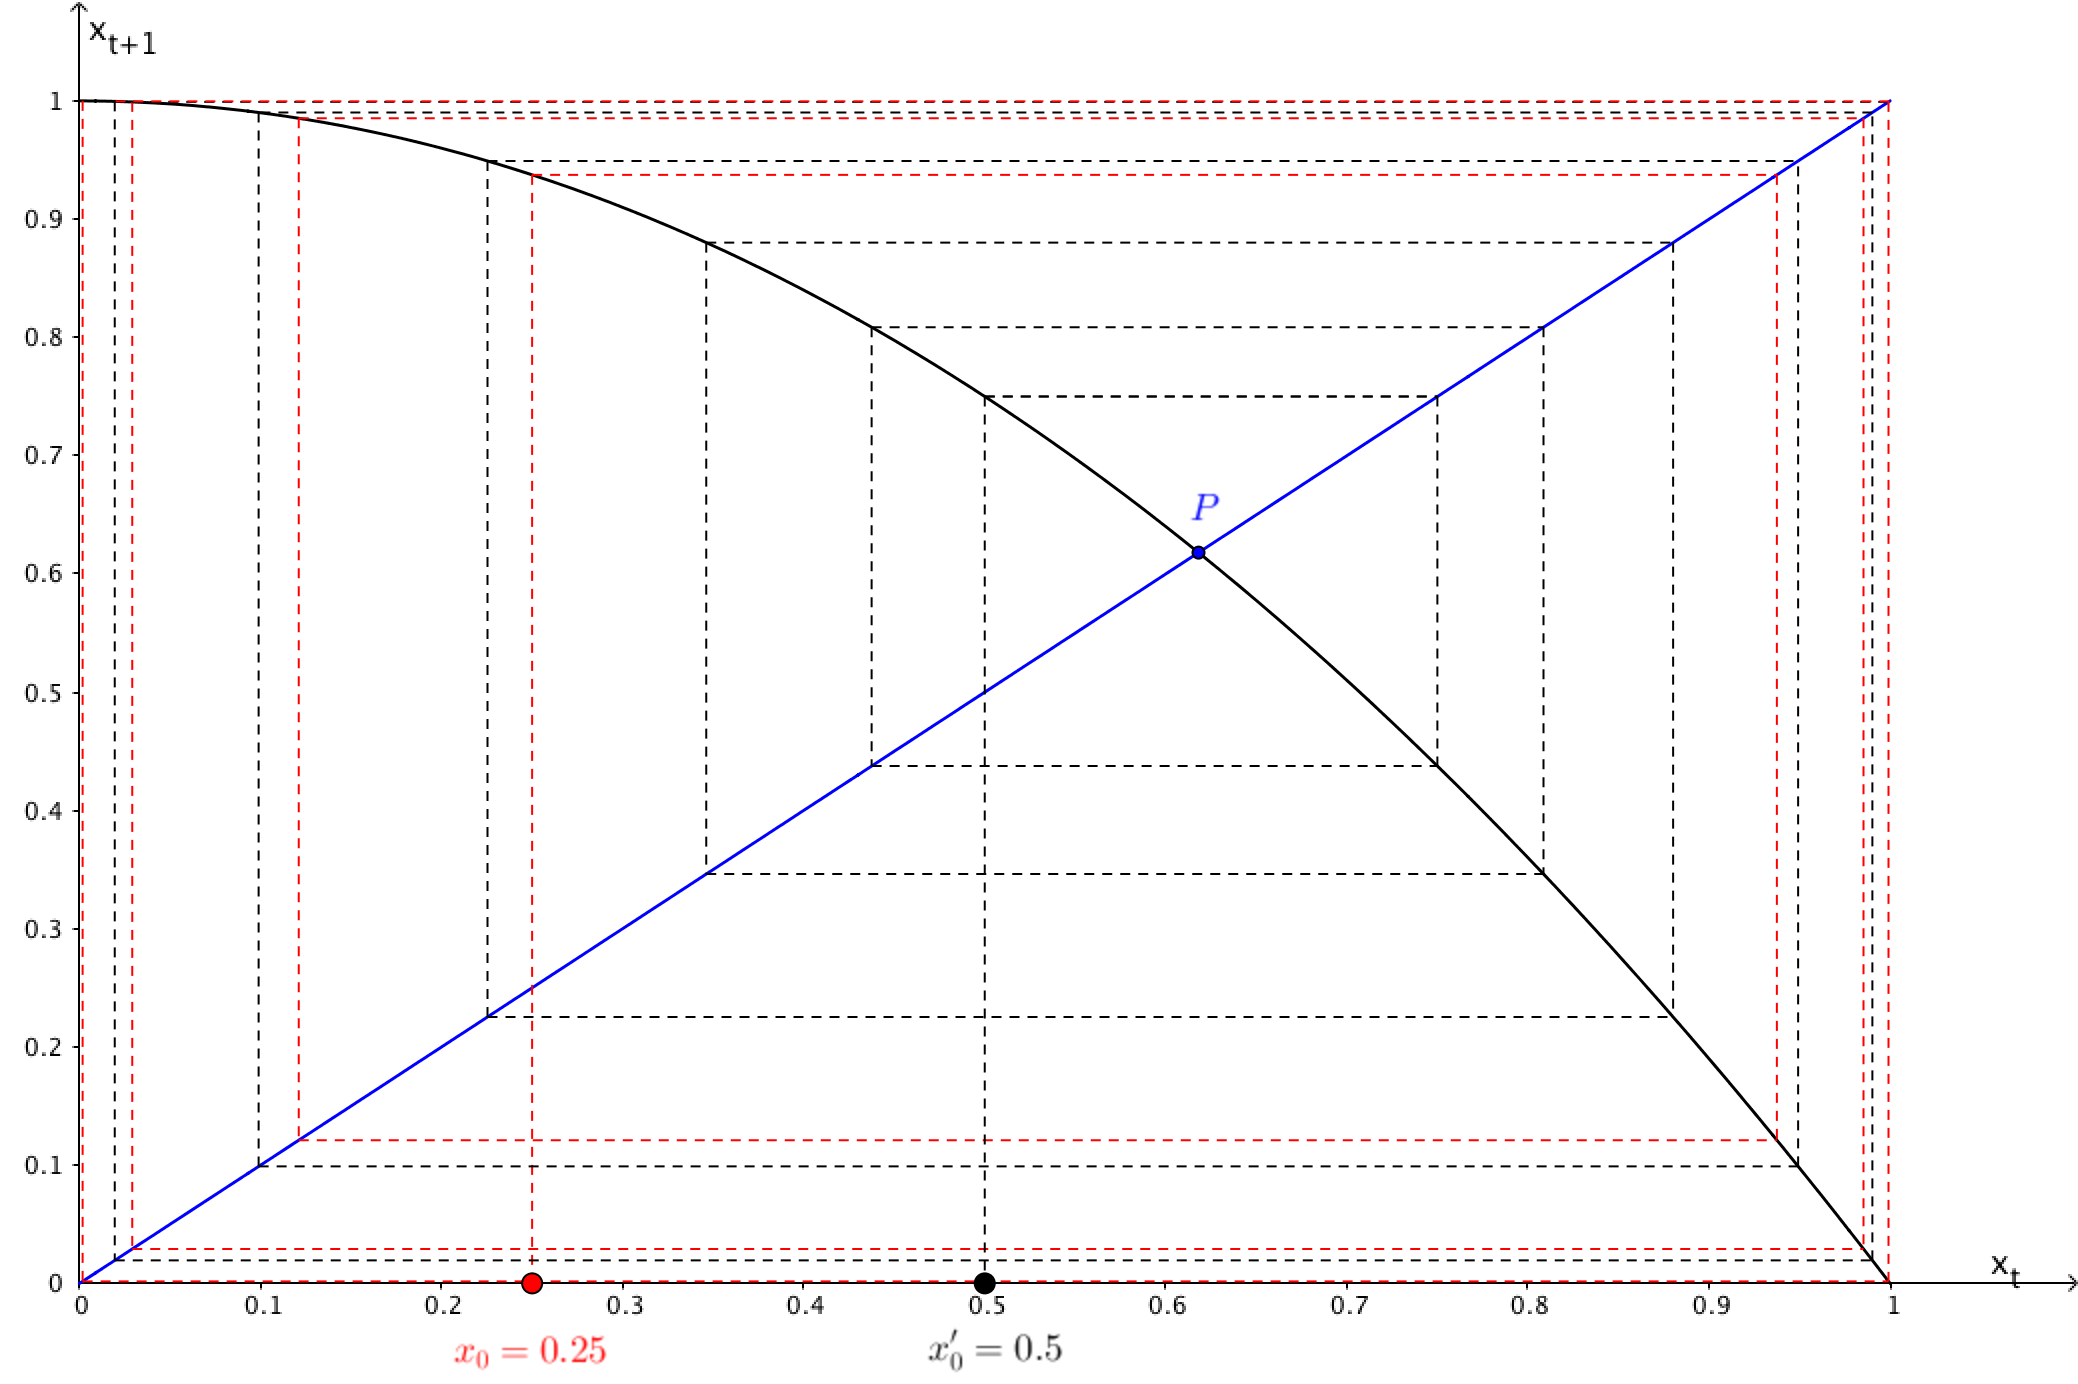
\includegraphics[width=\linewidth]{stable_graph_4.png}
		\end{figure}
		\end{center}


	\end{enumerate}

	\pagebreak


	\item Fiegenbaum's first constant is defined as 
	$$\lim_{k \to \infty}{\delta_k} = \delta = 4.669201 \dots $$
	with 
	$$\delta_k = \frac{a_k - a_{k-1}}{a_{k+1}-a_k}$$
	where $a_k$ corresponds to the $k^{th}$	bifurcation of the cascade of period-doubling bifurcations. By approximating $\delta_k \approx \delta$, the value of Feigenbaum's constant $\delta$ can be used to estimate other bifurcation parameters, $a_k$. 

	\begin{enumerate}
		\item The following diagram indicates the bifurcation pattern for the dynamical system $(1)$. The first interval, $0 \leq a < \frac{3}{4}$ of the graph indicates the interval over which all periodic orbits of period 1 are stable. The blue line indicates the bifurcation parameter $a_1 = \frac{3}{4}$ that determines the stability of period 1 orbits. The graph on the interval $\frac{3}{4} < a < \frac{5}{4}$ indicates the interval over which all periodic orbits of period 2 have stability. The red line indicates the value of the bifurcation parameter $a_2 = \frac{5}{4}$ which again, for a period 2 orbit, along with the parameter $a_1$, governs the stability of the period 2 orbits of the system. The yellow line indicates the parameter $a_3 = 1.357084703$, and the purple line indicates the important parameter $a_{\infty} = 1.386269449$, the value that determines the edge of chaos, and separates the values of $a$ for which orbits of period $n$ hold stability, and the values of $a$ for which the dynamical system degenerates to chaos.

		\begin{center}
		\begin{figure}[h!]
		\caption{$a$ vs $x$}
			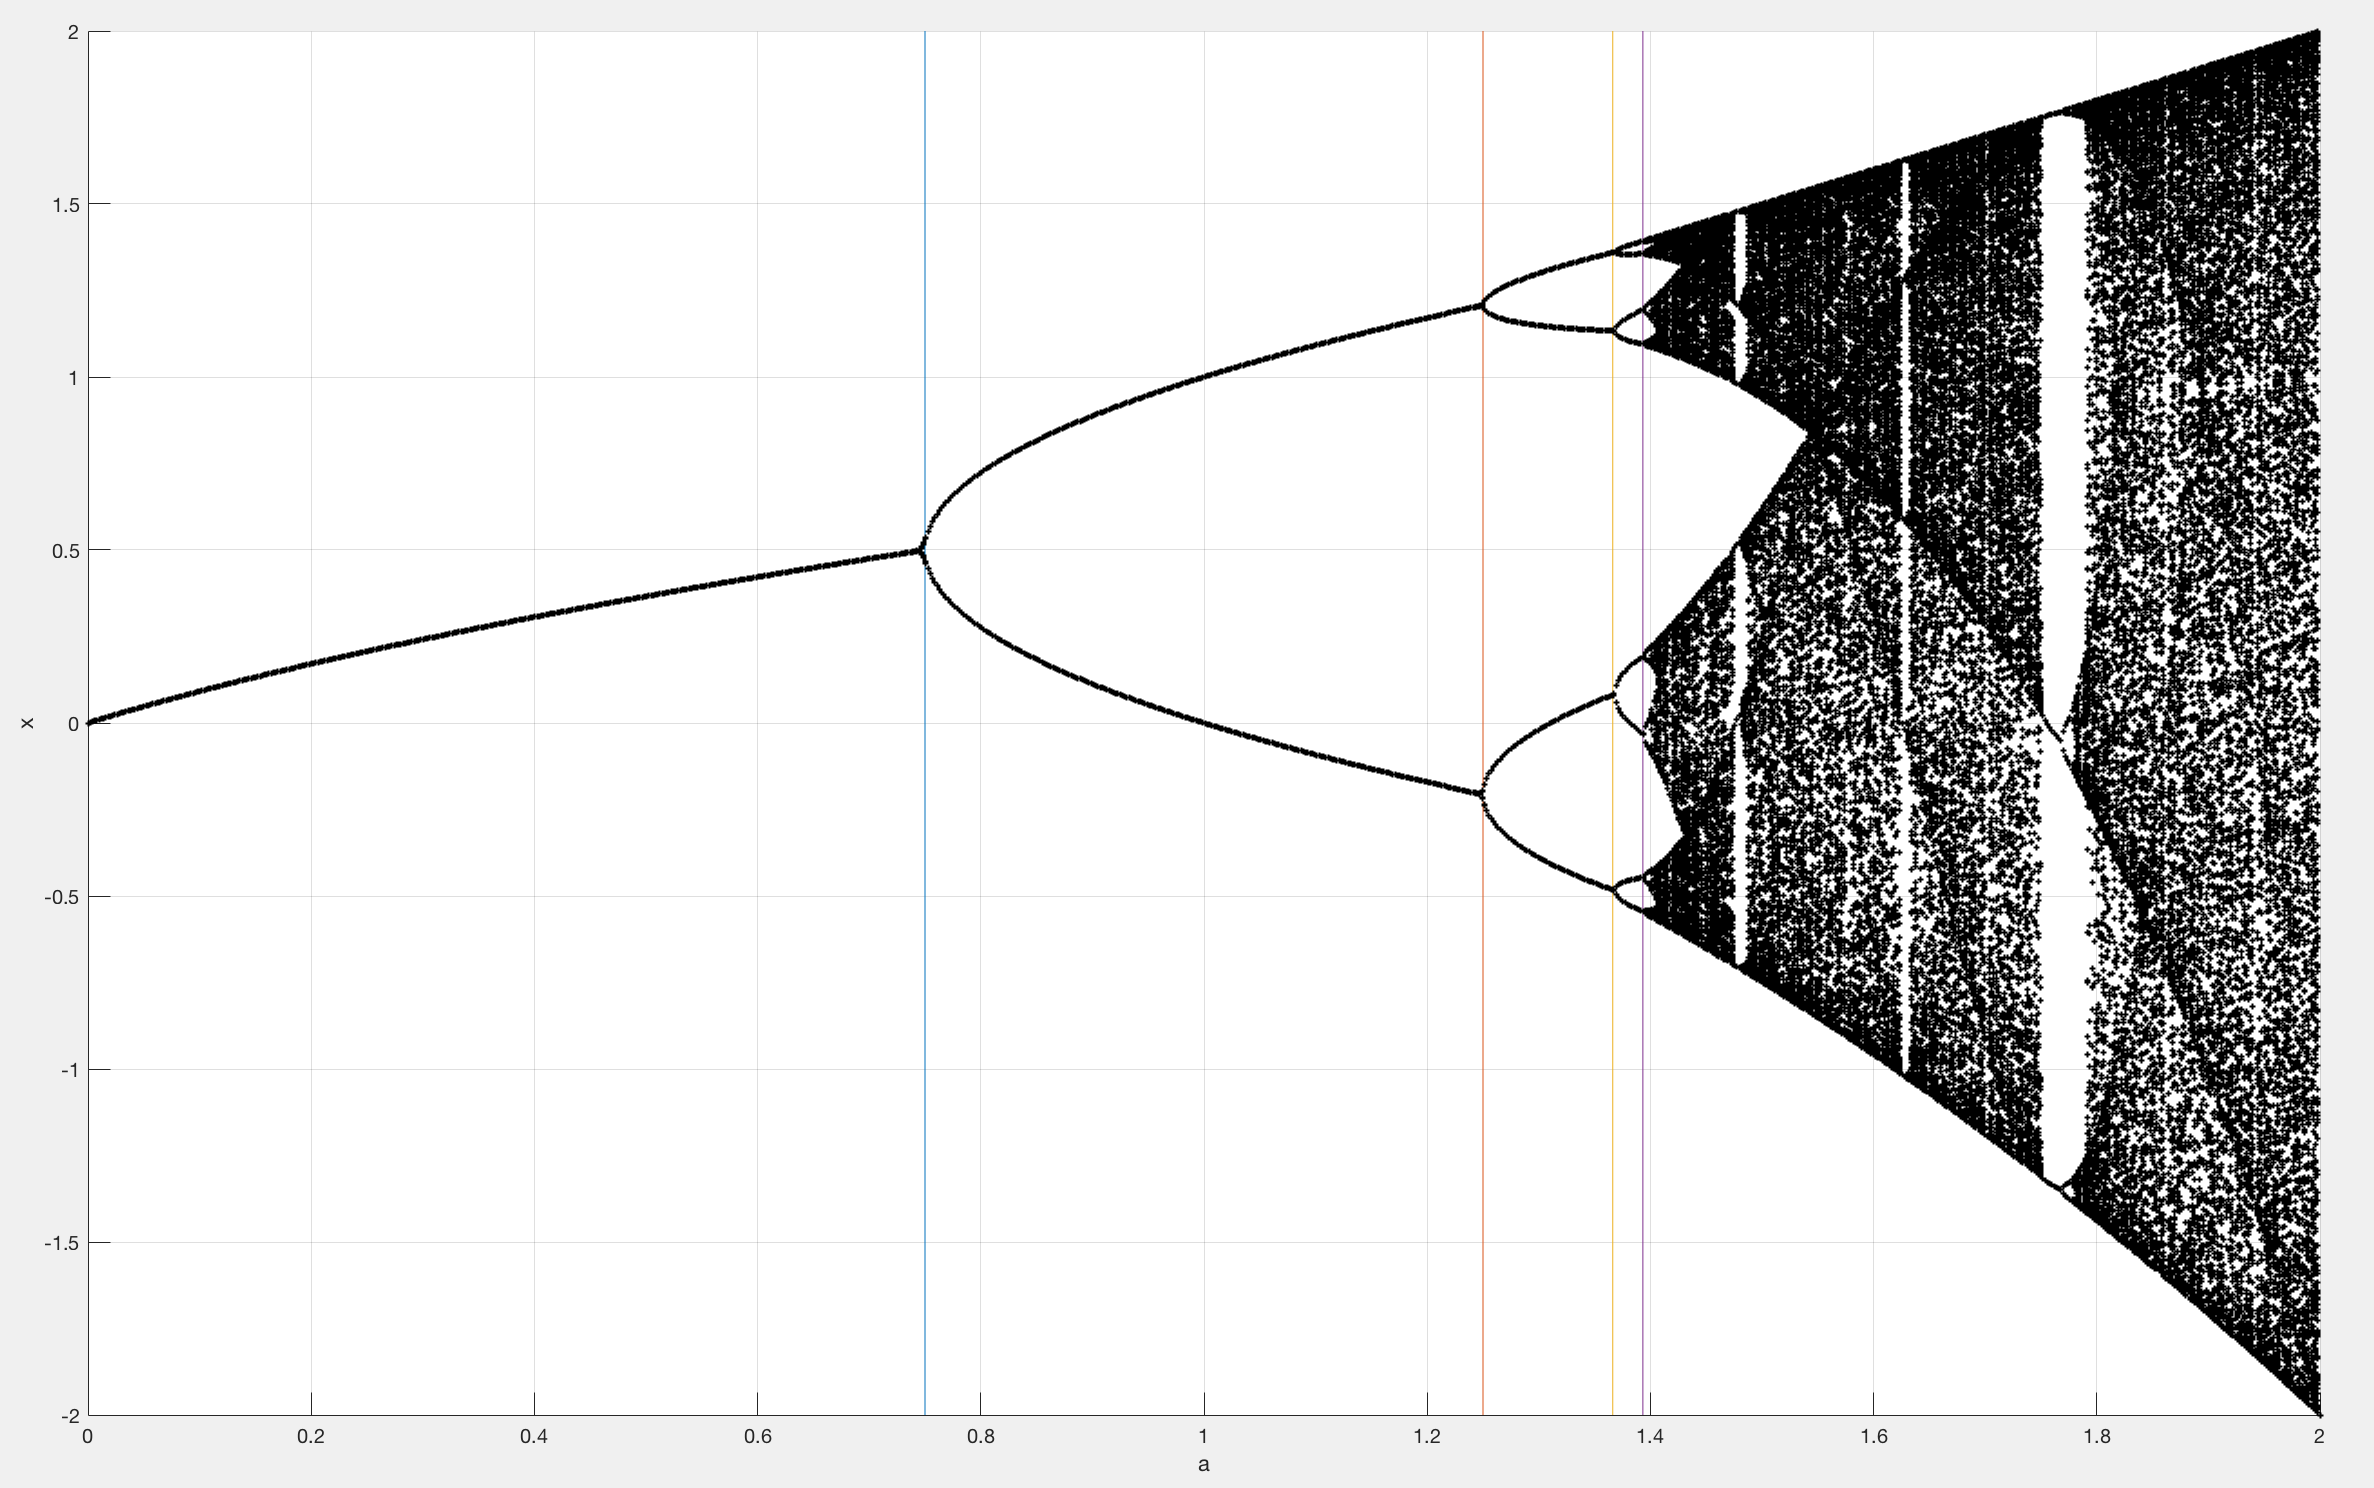
\includegraphics[width=\linewidth]{bifurcation_graph_3.png}
		\end{figure}
		\end{center}

		\pagebreak

		\item As $a_k$ is known as a bifurcation parameter, in other words, $a_k$ is the value at which the orbit of specific periodicity loses stabilty, we can use the intervals computed in the earlier questions to determine the bifurcation parameters $a_1$ and $a_2$. For the parameter $a_1$, the stability of orbits with period 1 disappears when $a$ takes the value $a_1 = \frac{3}{4}$. Subsequently, for the parameter $a_2$, the stabilty of period 2 orbits is lost when $a$ holds the value $a_2 = \frac{5}{4}$. Thus using these bifurcation parameters, and Fiegenbaum's first constant, we can compute the value of $a_3$.

		\begin{align*}
		\delta_k & = \frac{a_k - a_{k-1}}{a_{k+1}-a_k}\\
		\therefore \delta_2 & = \frac{a_2 - a_{1}}{a_{3}-a_2}\\
		\therefore \delta & = \frac{a_2 - a_{1}}{a_{3}-a_2} \hspace{5mm} \text{as } \delta_k = \delta\\
		\therefore a_{3}-a_2 & = \frac{a_2 - a_{1}}{\delta}\\
		\therefore a_3 & = \frac{a_2 - a_{1}}{\delta} + a_2\\
		& = \frac{\frac{5}{4} - \frac{3}{4}}{4.669201} + \frac{5}{4}\\
		\therefore a_3 & = 1.357084703\\
		\end{align*}

		\item In order to complete the derivation for $a_{\infty}$, we must first define $\displaystyle{\Delta_0 \coloneqq a_1 - a_0}$ and $\displaystyle{\Delta_k \coloneqq a_{k+1} - a_{k}}$. Thus as a result, the definition from above,
		$$\delta_k = \frac{a_k - a_{k-1}}{a_{k+1}-a_k}$$
		can be written as:
		$$\delta_k = \frac{\Delta_{k-1}}{\Delta_{k}}$$

		

		Now to derive the value for $a_{\infty}$, we will progress as follows below, first examining the infinite product.

		\begin{align*}
		\delta_1 \delta_2 \delta_3 \dots \delta_k & = \prod_{k=1}^{\infty}\delta_k\\
		& = \prod_{k=1}^{\infty}\frac{\Delta_{k-1}}{\Delta_{k}}\\
		& = \left[\frac{\Delta_0}{\Delta_{1}}\right] \left[\frac{\Delta_1}{\Delta_{2}}\right] \left[\frac{\Delta_2}{\Delta_{3}}\right] {\dots} \left[\frac{\Delta_{k-1}}{\Delta_{k}}\right]\\
		\therefore \delta_1 \delta_2 \delta_3 \dots \delta_k & = \frac{\Delta_0}{\Delta_{k}}\\
		\therefore \delta \delta \delta \dots \delta & = \frac{\Delta_0}{\Delta_{k}}\\
		\therefore \delta^{k} & = \frac{\Delta_0}{\Delta_{k}}\\
		\therefore \Delta{k} & = \frac{\Delta_0}{\delta^{k}}\\
		\end{align*}

		\begin{align*}
		\therefore a_{k+1} - a_k & = \frac{\Delta_0}{\delta^{k}} \hspace{5mm} \text{by definition}\\
		\therefore a_{k+1} & = \frac{\Delta_0}{\delta^{k}} + a_k\\
		& = \frac{\Delta_0}{\delta^{k}} + \frac{\Delta_0}{\delta^{k-1}} + a_{k-1}\\
		\therefore a_{\infty} & = \frac{\Delta_0}{\delta^{k}} + \frac{\Delta_0}{\delta^{k-1}} + \frac{\Delta_0}{\delta^{k-2}} + \dots + \frac{\Delta_0}{\delta^{1}} + a_1\\
		& = \Delta_0 \left[\frac{1}{\delta^{k}} + \frac{1}{\delta^{k-1}} + \frac{1}{\delta^{k-2}} + \dots + \frac{1}{\delta^{1}} \right] + a_1\\
		& = \Delta_0 \left[\sum_{k=1}^{\infty}\frac{1}{\delta^{k}} \right] + a_1\\
		& = \Delta_0 \left[\frac{\frac{1}{\delta}}{1-\frac{1}{\delta}} \right] + a_1\\
		& = \Delta_0 \left[\frac{\frac{1}{\delta}}{\frac{\delta - 1}{\delta}} \right] + a_1\\
		& = \Delta_0 \left[\frac{1}{\delta - 1} \right] + a_1\\
		& = \frac{\delta}{\Delta_1} \left[\frac{1}{\delta - 1} \right] + a_1 \hspace{5mm} \text{as } \delta_1 = \frac{\Delta_{0}}{\Delta_{1}} \text{ and } \delta_1 = \delta\\
		\therefore a_{\infty} & = \Delta_1 \left[\frac{\delta}{\delta - 1} \right] + a_1 \\
		\therefore a_{\infty} & = \left[a_2 - a_1 \right] \left[\frac{\delta}{\delta - 1} \right] + a_1 \\
		\therefore a_{\infty} & = \left[\frac{5}{4} - \frac{3}{4} \right] \left[\frac{\delta}{\delta - 1} \right] + \frac{3}{4} \hspace{5mm} \text{as } \Delta_1 = a_2 - a_1\\
		\therefore a_{\infty} & = \frac{1}{2} \left[\frac{\delta}{\delta - 1} \right] + \frac{3}{4}\\
		\therefore a_{\infty} & = \frac{\delta}{2\left(\delta - 1 \right)} + \frac{3}{4}\\
		\therefore a_{\infty} & = \frac{4.669201}{2\left(4.669201 - 1 \right)} + \frac{3}{4}\\
		\therefore a_{\infty} & = 1.386269449\\
		\end{align*}










	\end{enumerate}








\end{enumerate}

\end{document}